%% Compile me as follows:
%%% latexmk -pdf -xelatex -shell-escape presentation.tex

\documentclass[xetex,compress]{beamer}
%% \usetheme{Pittsburgh}
%% \usecolortheme{seagull}

%% https://www.quora.com/Presentations-What-are-the-best-beamer-themes
\setbeamertemplate{frametitle}
  {\begin{centering}\smallskip
   \insertframetitle\par
   \smallskip\end{centering}}
\setbeamertemplate{itemize item}{\(\bullet\)}
\setbeamertemplate{navigation symbols}{}
\setbeamertemplate{footline}[text line]{%
    \hfill\strut{%
        \scriptsize\sf\color{black!60}%
        \quad\insertframenumber
    }%
    \hfill
}
%% \setbeamertemplate{caption}{\raggedright\insertcaption\par}

% Define some colors:
\definecolor{PittBlue}{RGB}{0,43,94}
\definecolor{PittGold}{RGB}{197,168,118}
\definecolor{DarkFern}{HTML}{407428}
\definecolor{DarkCharcoal}{HTML}{4D4944}
\colorlet{Fern}{DarkFern!85!white}
\colorlet{Charcoal}{DarkCharcoal!85!white}
\colorlet{LightCharcoal}{Charcoal!50!white}
\colorlet{AlertColor}{orange!80!black}
\colorlet{DarkRed}{red!70!black}
\colorlet{DarkBlue}{blue!70!black}
\colorlet{DarkGreen}{green!70!black}
% Use the colors:
\setbeamercolor{title}{fg=PittBlue}
\setbeamercolor{frametitle}{fg=PittBlue}
\setbeamercolor{normal text}{fg=DarkCharcoal}
\setbeamercolor{block title}{fg=black,bg=Fern!25!white}
\setbeamercolor{block body}{fg=black,bg=Fern!25!white}
\setbeamercolor{alerted text}{fg=AlertColor}
\setbeamercolor{itemize item}{fg=Charcoal}

\usepackage[utf8]{inputenc}
\usepackage[T1]{fontenc}
\usepackage{alltt}
\usepackage{bm}
\usepackage[normalem]{ulem}
\usepackage{paralist}
\usepackage{setspace}
\usepackage{xparse}
\usepackage{braket}
\usepackage{wrapfig}
\usepackage[export]{adjustbox}

\makeatletter
\g@addto@macro\@floatboxreset\centering
\makeatother

\DeclareDocumentCommand{\vect}{m}{
        \ensuremath{\boldsymbol{\mathbf{#1}}}
}

%%% Chemistry
\usepackage{chemformula}

\makeatletter
\newcommand\listofframes{\@starttoc{lbf}}
\makeatother

\addtobeamertemplate{frametitle}{}{%
  \addcontentsline{lbf}{section}{\protect\makebox[2em][l]{%
    \protect\usebeamercolor[fg]{structure}\insertframenumber\hfill}%
  \insertframetitle\par}%
}

\setbeamertemplate{navigation symbols}{}

%%%%%%%%%%%%%%%%%%%%%%%%%%%%%%%%%%%%%%%%%%%%%%%%%%%%%%%%%%%%%%%%%%%%%%%%%%%%%%

\title{Deciphering the Contents of Chemically-Trained Neural Networks into Physical Intuition}
\author[Berquist]{Eric Berquist}
%% \institute[Pitt]{University of Pittsburgh}
\institute[Pitt]{
\includegraphics[width=1in]{./logo.png}}
\date{June 15th, 2017}

\begin{document}

\frame{
  \titlepage
}

%% \begin{frame}{Outline}
%%   \tableofcontents
%% \end{frame}

\begin{frame}{Roadmap}
  \begin{itemize}
  \item Quantum chemical calculations of EPR parameters aid in the
    interpretation and rationalization of experimental results
  \item DFT calculations of EPR \textit{g}-tensors for \ch{Cu^{2+}}
    systems show large deviations from experimental measurements and
    between different density functionals
  \item Understanding the differences in electronic structure between
    DFT and benchmark-quality wavefunction methods is necessary for
    proposing improvements to DFT
  \item Hypothesis: Parametrization of DFT is a viable method for
    improvement
  \end{itemize}
\end{frame}

\begin{frame}{Literature Survey}
  In published work, how do \textit{g}-tensors calculated using
  density functional theory of \ch{Cu^{2+}}-containing systems compare
  to experimental results?
\end{frame}

\begin{frame}{Methodology of the Literature Analysis}
  For each paper:
  \begin{itemize}
  \item Extract available parameters: \(g_{xx}\),
    \(g_{yy}\),
    \(g_{zz}\),
    \(g_{11}\),
    \(g_{22}\),
    \(g_{33}\), \(g_{\perp}\), \(g_{\parallel}\), \(g_{\text{iso}}\)
  \item Where there are multiple calculations for one experimental
    data point, use the one with best agreement
  \item Calculate missing values of \(g_{\parallel}\),
    \(g_{\text{iso}}\), and \(g_{\perp}\)if possible
  \end{itemize}
  \vspace{\baselineskip} For each of \(g_{\parallel}\),
  \(g_{\text{iso}}\), and \(g_{\perp}\):
  \begin{itemize}
  \item Perform linear regression for the set of points
  \item Calculate the ``percent incorrect trend''
  \end{itemize}
\end{frame}

%% \begin{frame}
%% \end{frame}

\begin{frame}{What is machine learning}
  Arthur Samuel, 1959, the subfield of computer science that gives:
  \begin{quote}
    computers the ability to learn without being explicitly programmed.
  \end{quote}
  \begin{quote}
    A computer program is said to learn from experience \textit{E} with respect to some class of tasks \textit{T} and performance measure \textit{P} if its performance at tasks in \textit{T}, as measured by \textit{P}, improves with experience \textit{E}.
  \end{quote}
\end{frame}

\begin{frame}{}
  \begin{center}
    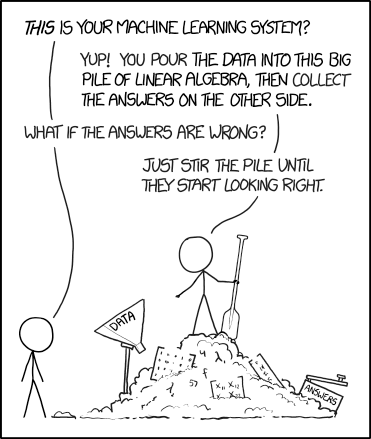
\includegraphics[width=0.75\textwidth]{./machine_learning.png}
  \end{center}
\end{frame}

\begin{frame}{}
  \begin{center}
    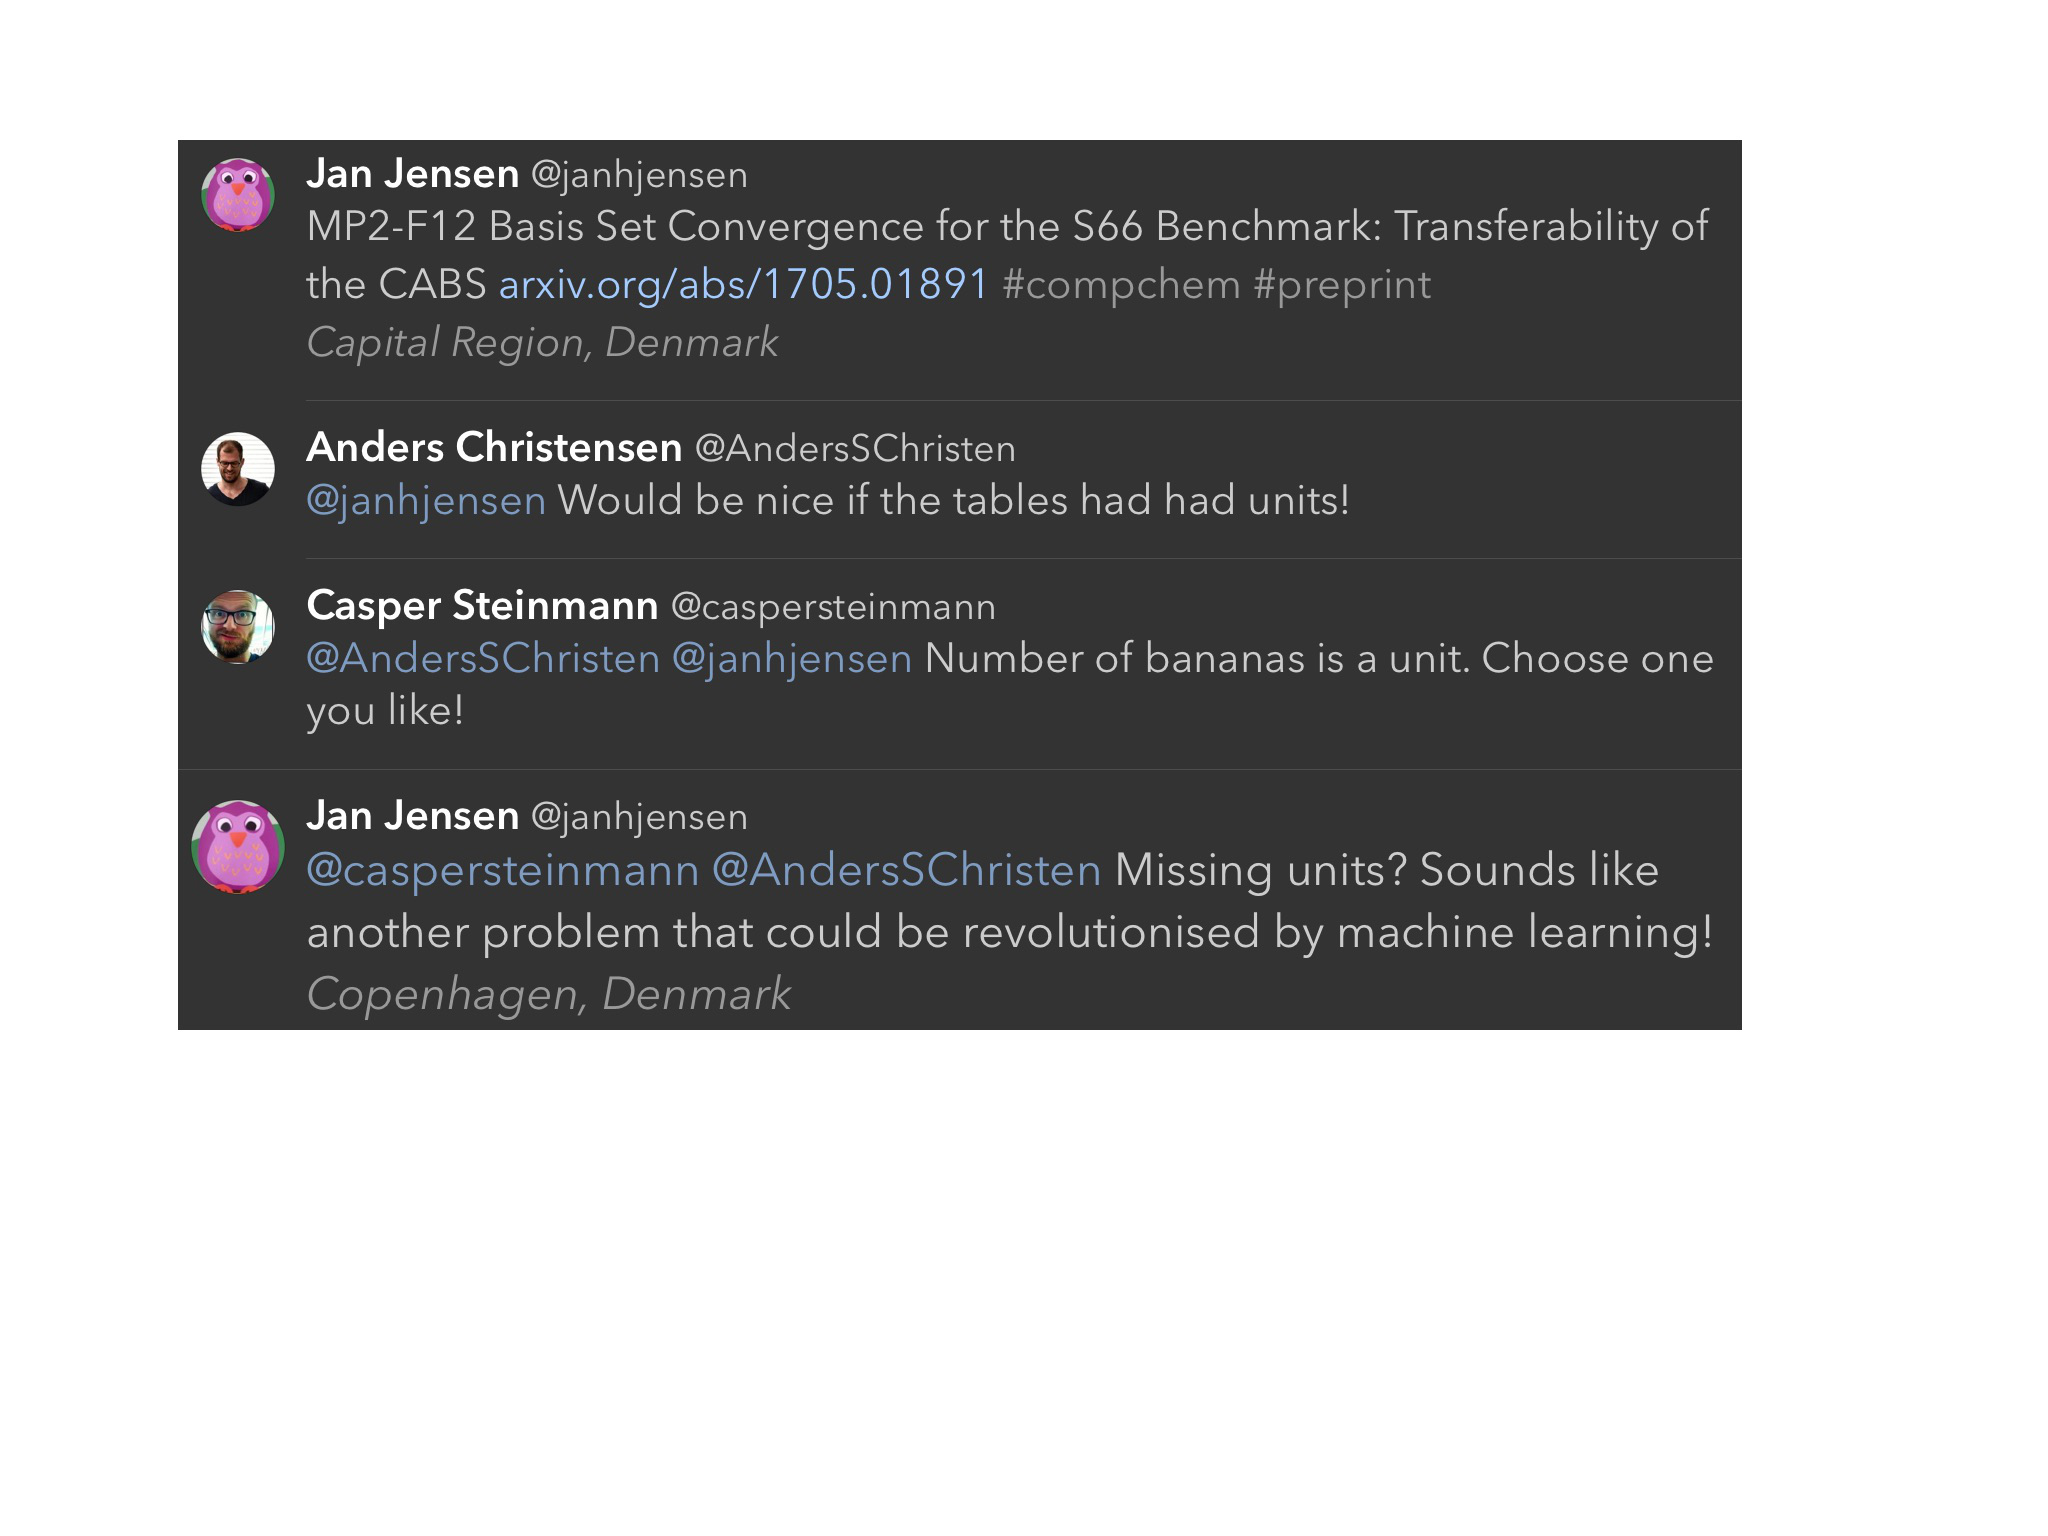
\includegraphics[width=1.10\textwidth]{./twitter.jpeg}
  \end{center}
\end{frame}

\begin{frame}{An (imperfect) analogy between neural networks and quantum chemistry}
  \begin{itemize}
  \item The fundamental components of the network (kind of neuron activation functions, convolution or direct connection) are like the \emph{Hamiltonian}.
  \item The number of components in each network layer and the number of layers are like the size of the \emph{basis set}.
  \end{itemize}
\end{frame}

\begin{frame}{A better analogy}
  between relevance propagation and interaction energy decomposition approaches (SAPT, EDA):
  \begin{itemize}
  \item I am an item
  \end{itemize}
\end{frame}

%% Changing the number of layers and number of nodes per layer is like altering the variational upper bound of the network
%% Weights are like MO coefficients

%% Review of the relevant literature I missed: ANI-1, DTNN

\begin{frame}{Definitions of trained molecular properties}
  \begin{itemize}
  \item Zero-point (vibrational) energy: \(E_{\text{ZPVE}} = \frac{1}{2} h \sum_{i}^{\text{normal modes}} \nu_{i}\)
  \item Isotropic polarizability (static, \(\omega = 0\)): \(\alpha_{\text{iso}} = \bar{\alpha} \equiv \frac{1}{3} (\alpha_{xx} + \alpha_{yy} + \alpha_{zz})\)
  \item Parallel 1st hyperpolarizability (static, \(\omega_{a} = \omega_{b} = 0\)): \(\beta_{\parallel} \equiv\)
  \end{itemize}
\end{frame}

%% \begin{frame}{}
%% \fxnote{Also, what to do in the event that the lit model isn't reproducible? It may indicate that not enough information is given in the literature: publications are notorious for not providing enough information about code/model parameters for reproduction. Even in the event of supposed failure to fall within the error metric, the architecture is still a valuable building block. Is it safe to assume that the PI (me) will not make any mistakes in the implementation? Another possible point of failure may be due to the non-convex optimization problem posed by NNs. What is the likelihood of training a network into a local minimum?}
%% \end{frame}

\begin{frame}{Timeline}
\end{frame}

\begin{frame}{A future challenge: building databases}
  \begin{itemize}
  \item GDB9/QM9 is the most commonly-used training set, the equivalent of the MNIST set of \~10,000 labeled handwritten digits.
  \item It is now suffering from the same problem as MNIST: it is too simple and not representative of real-world training cases (molecules).
  \item Analogy: Pople basis sets (6-31G and derivatives) are still extremely common, not even because we don't know better, but because we ``need to compare to past work''.
  \item If a \emph{general and transferable} ML model fails on GDB9, that is a warning sign, but the above cannot be a reason against extending deeper into chemical space for ML model training.
  \end{itemize}
\end{frame}

\begin{frame}{Backup Slides}
\end{frame}

\begin{frame}{Hyperpolarizability equations from paper}
  When the dipole moment coincides with the \(j\)-axis, we have
  \begin{equation}
    \beta_{\parallel} = \frac{3}{5}\beta_j = \frac{1}{5} \sum_{i=x,y,z} (\beta_{iij} + \beta_{iji} + \beta_{jii}),
  \end{equation}
  or in the general case,
  \begin{equation}
    \beta_{\parallel} = \frac{3}{5|\mu|} \sum_{i,j=x,y,z} \beta_{iij} \mu_{j},
  \end{equation}
  where
  \begin{equation}
    \beta_{ijk} = \left<\left<\mu_{i};\mu_{j},\mu_{k}\right>\right>.
  \end{equation}
\end{frame}

\end{document}
